

\documentclass[a4paper, 11pt]{article}
\usepackage[czech]{babel}
\usepackage[utf8]{inputenc}
\usepackage[left=2cm, top=3cm, text={17cm, 24cm}]{geometry}
\usepackage{times}
\usepackage{verbatim}
\usepackage{enumitem}
\usepackage{amsmath, bm}
\usepackage{svg}
\usepackage[graphicx]{realboxes}
% \usepackage[unicode]{hyperref}
\usepackage[hidelinks]{hyperref}
\usepackage{xurl}
\usepackage{array, tabularx}

% \usepackage{bera}
\usepackage{listings}
\usepackage{xcolor}

\colorlet{punct}{red!60!black}
\definecolor{background}{HTML}{EEEEEE}
\definecolor{delim}{RGB}{20,105,176}
\colorlet{numb}{magenta!60!black}

\lstdefinelanguage{json}{
    basicstyle=\normalfont\ttfamily,
    numbers=none,
    numberstyle=\scriptsize,
    stepnumber=1,
    numbersep=8pt,
    showstringspaces=false,
    breaklines=true,
    frame=lines,
    backgroundcolor=\color{background},
    %  *{0}{{{\color{numb}0}}}{1}
    %   {1}{{{\color{numb}1}}}{1}
    %   {2}{{{\color{numb}2}}}{1}
    %   {3}{{{\color{numb}3}}}{1}
    %   {4}{{{\color{numb}4}}}{1}
    %   {5}{{{\color{numb}5}}}{1}
    %   {6}{{{\color{numb}6}}}{1}
    %   {7}{{{\color{numb}7}}}{1}
    %   {8}{{{\color{numb}8}}}{1}
    %   {9}{{{\color{numb}9}}}{1}
    literate=
      *{:}{{{\color{punct}{:}}}}{1}
      {,}{{{\color{punct}{,}}}}{1}
      {\{}{{{\color{delim}{\{}}}}{1}
      {\}}{{{\color{delim}{\}}}}}{1}
      {[}{{{\color{delim}{[}}}}{1}
      {]}{{{\color{delim}{]}}}}{1},
}


\begin{document}

\begin{sloppypar}
\begin{titlepage}
		\begin{center}
			
\includegraphics[width=0.85\linewidth]{./figs/logo_cz.png} \\

			\vspace{\stretch{0.382}}

			\Huge{Dokumentace k~projektu} \\
			\LARGE{\textbf{PCAP Netflow v5 exportér}} \\
			\vspace{\stretch{0.61}}
		\end{center}

			\Large

   
            \begin{tabularx}{0.96\textwidth}{ll>{\raggedleft\arraybackslash}X}
                \textbf{Jakub Gryc} & \texttt{xgrycj03} &  \Large\today \\ 
                 %&  &  & \\ 
                %\textbf{FUNEXP} & \ &  &  
			\end{tabularx}


        % \end{minipage}
	\end{titlepage}

\tableofcontents

\newpage
\section{Úvod}

Cílem projektu bylo vytvořit aplikaci, která bude schopna zpracovávat soubory ve formátu PCAP a~na základě těchto souborů generovat Netflow záznamy ve verzi 5. Tyto záznamy jsou následně posílány pomocí transportního protokolu UDP na kolektor. Aplikace je napsána v~jazyce C++ a~využívá knihovnu \texttt{libpcap} pro zpracování PCAP souborů.
\section{Návrh a~implementace}

Aplikace je rozdělena do několika tříd a souborů, které vzájemně spolupracují. Veškeré zdrojové soubory jsou umístěny v~adresáři \texttt{src/}. Některé důležité třídy a~jejich metody jsou popsány v~následujících podkapitolách.
\subsection{Vstupní bod programu, main.cpp}
Soubor \texttt{main.cpp} obsahuje vstupní bod programu. V~této části se zpracovávají argumenty a inicializují se hlavní třídy programu. Jedna z těchto tříd je třída Timer, která si po své inicializaci uloží časovou značku, která je nadále využívána pro výpočet relativního času v~Netflow záznamech. Dále se zde inicializuje třída UDPConnection, která obstarává posílaní UDP zpráv na kolektor. Poslední třídou, která je zde inicializována, je třída PcapHandler, která slouží jako hlavní jádro celé aplikace, jejíž účel je popsán v další podkapitole.
\subsection{Zpracování paketů - PcapHandler}
Hlavní jádro programu se nachází ve třídě PcapHandler. Po své inicializaci otevře PCAP soubor a~postupně zpracovává jednotlivé pakety. Metoda \texttt{PcapHandler::start()} inicializuje instanci třídy FlowCache, která slouží jako rozhraní pro ukládání a manipulování s uloženými Netflow záznamy. Následně se iteruje přes každý paket v~PCAP souboru a~volá se metoda \texttt{PcapHandler::processPacket()}, která zpracovává jednotlivé pakety a relevantní informace z~nich ukládá do FlowCache. Po zpracování všech paketů se zavolá metoda \texttt{PcapHandler::sendFlows()}, která postupně prochází všechny uložené Netflow záznamy a~tyto záznamy odesílá na kolektor pomocí třídy UDPConnection. Pokud vypršel aktivní či neaktivní časový limit pro 30 a více záznamů, tak se tyto záznamy po 30 mohou na kolektor odeslat ještě dříve, než se zpracují všechny pakety v~PCAP souboru. Tato funkcionalita je více popsána později viz \ref{timelimits}.

\subsection{Zpracování netflow záznamů - FlowCache}
Tato třída uchovává jednotlivé záznamy ve formě hash tabulky. Každý záznam je identifikován pomocí klíče, který je složen ze zdrojové IP adresy a portu a cílové IP adresy a portu. Transportní protokol se neukládá, jelikož aplikace řeší jen záznamy o TCP tocích. Hodnoty v této tabulce pak tvoří struktura Flow, která obsahuje informace jako počet bytů, počet paketů, čas prvního a posledního záznamu a další. Třídy FlowCache a Flow obsahují metody pro přidání nového záznamu, aktualizaci stávajícího záznamu či odeslání všech záznamů na kolektor.

\subsubsection*{Časové limity} \label{timelimits}
Důležitou součástí je hlídání časových limitů pro jednotlivé záznamy. Před každou aktualizací FlowCache se kontroluje, zda jednotlivým záznamům nevypršel časový limit. Veškeré expirované záznamy se odstraní z tabulky a přiřadí do fronty \verb|exportCache|. Do fronty se záznamy přidávají vždy podle toho, jak dlouho je záznam expirovaný. Nejdéle expirované záznamy se do fronty přidávají jako první, jak je popsáno v  \cite{flows}, sekce V-C, aby byly poslány dříve. Funkcionalitu zajišťuje metoda \texttt{FlowCache::checkForExpiredFlows()}.

Exportované záznamy se už přímo ukládají do struktury, která se pošle na kolektor. Je zajištěno správné pořadí bytů a~tedy jejich konverze do síťového bytového pořadí.


\begin{figure}[ht]
    \begin{center}
        \scalebox{0.9}{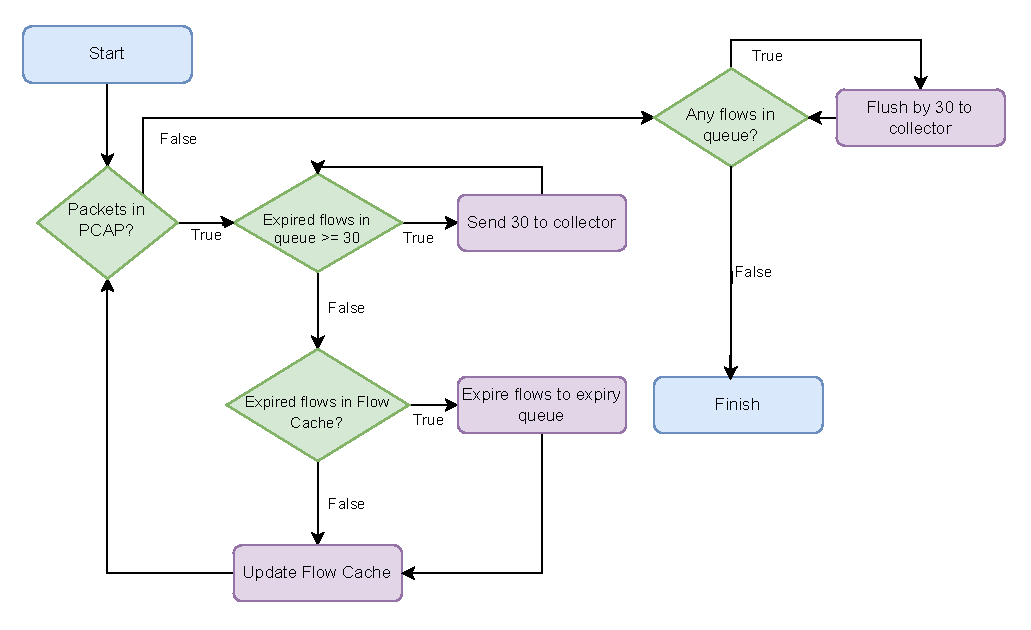
\includegraphics{./figs/flowchart.drawio.pdf}}
        \caption{Diagram zpracování paketů a~odesílání Netflow záznamů mého exportéru.}
        \label{fig1}
    \end{center}
\end{figure}


\subsection{UDP spojení}
Třída UDPConnection slouží k~odesílání Netflow záznamů na kolektor. Po své inicializaci se vytvoří socket, který je následně využíván pro odesílání záznamů. Metoda \texttt{UDPConnection::sendFlows()} odesílá postupně jednotlivé záznamy na kolektor v Netflow v5 formátu \cite{netflow5}. Pokud ještě nedošlo ke zpracování všech paketů ze souboru, tak se záznamy odesílají jen po 30 záznamech, které byly již exportovány do \verb|exportCache|. Pokud jich je méně, tak se záznamy neposílají a čeká se na naplnění fronty na alespoň 30 záznamů. Pokud se zpracovaly všechny pakety, tak se záznamy posílají všechny, i když jich je méně než 30, postupně po 30.

\section{Návod k~použití}

Program je možné sestavit pomocí příkazu \texttt{make} v domovském adresáři projektu. Po sestavení je možné program spustit s~následujícími argumenty:

\vspace{0.1cm}
\texttt{
    ./p2nprobe <host>:<port> <pcap\_file> [-a <active\_timeout>] 
            [-i <inactive\_timeout>]
}

\begin{itemize}
    \item \texttt{<host>:<port>} - povinný argument, který určuje IP adresu a port, na kterých kolektor běží.
    \item \texttt{<pcap\_file>} - povinný argument, který určuje cestu k PCAP souboru, který se analyzuje.
    \item \texttt{-a <active\_timeout>} - nepovinný argument, který určuje časový limit pro aktivní timeout. Výchozí hodnota je 60 sekund.
    \item \texttt{-i <incative\_timeout>} - nepovinný argument, který určuje časový limit pro neaktivní timeout. Výchozí hodnota je 60 sekund.
\end{itemize}

\section{Testování}
Pro korektní testování bylo nutné obstarat si několik PCAP souborů. Pro testování základní funkčnosti exportéru jsem si vytvořil dva jednoduché programy v Pythonu, jeden sloužil jako TCP klient a druhý jako TCP server. Tyto programy jsem spustil a zachytil jejich komunikaci pomocí nástroje Wireshark, kterou jsem ukládal do PCAP souborů. Jejich implementace je dostupná v adresáři \texttt{tests/}, PCAP soubory v \texttt{tests/pcaps}. Implementoval jsem taktéž jednoduchý testovací skript \texttt{tests/test.py} v Pythonu, který obsahuje mnou implemntovaný kolektor. Tento skript pouští můj exportér a kolektor, který následně zpracovává přijaté záznamy a ukládá je do logů v adresáří \texttt{tests/logs}. Takto jsem byl schopen jednoduše ověřovat obsah záznamů, které exportér posílá.

Logy z kolektoru jsou ve formátu JSON a obsahují dvě pole, \texttt{headers} a \texttt{records}. Pole \texttt{received} obsahuje hlavičky záznamů, které kolektor přijal, a pole \texttt{records} obsahuje samotné záznamy. Záznamy rovněž obsahují zpracovanou časovou značku, kdy byl záznam odeslán a délku trvání flowu, tyto hodnoty exportér neodesílá.

% insert json example of log
\begin{lstlisting}[language=json, caption={Ukázka logu z kolektoru}, label={lst1}]
{
    "headers": {
        "header_0": {
            "Version": 5,
            "Count": 2,
            "SysUptime": 0,
            "UnixSecs": 1731704591,
            "UnixNsecs": 808015000,
            "FlowSequence": 0,
            "EngineType": 0,
            "EngineID": 0,
            "SamplingInterval": 0
        }
    },
    "records": {
        "0184c1408f81a885a9bbdb50fc88065a": {
            "Timestamp": "2024-10-14 00:38:17.370",
            "SrcAddr": "127.0.0.1",
            "DstAddr": "127.0.0.1",
            "NextHop": "0.0.0.0",
            "Input": 0,
            "Output": 0,
            "Packets": 4,
            "Octets": 216,
            "First": 1449472857,
            "Last": 1449491651,
            "Duration": 18794,
            "SrcPort": 9119,
            "DstPort": 14002,
            "Padding": 0,
            "TCPFlags": 19,
            "Protocol": 6,
            "Tos": 0,
            "SrcAS": 0,
            "DstAS": 0,
            "SrcMask": 0,
            "DstMask": 0,
            "Padding2": 0
        },
        ...
    }
}

\end{lstlisting}


Program rovněž obsahuje několik testů, které pouští jak můj exportér, tak referenční exportér \texttt{softflowd} a porovnává jejich výstupy. Tyto testy lze spustit pomocí příkazu \texttt{python test.py -c -r}. Vzhledem k tomu, že referenční exportér má jinou implementaci, není možné jej plnohodně porovnávat s naším zadáním. Softflowd například nedokáže měnit časové limity, když načítá pakety ze souboru, taktéž řeší TCP fin a reset flagy. To v našem našem exportéru není zadáno. Testy tedy spíš slouží k porovnání jen se soubory, které obsahují malé množství záznamů, kdy se výstupy téměř vždy shodují.
\section{Závěr}

\bibliography{citations}
\bibliographystyle{czechiso}
\end{sloppypar}
\end{document}
